\msusection{Output Menu}
\msusubsection{Output data to file(s)}
The weather data from YCweather may be exported as a comma separated text (*.txt), Microsoft Excel 97-2003 (*.xls), or Microsoft Excel 2007 (*.xlsx) file via the Output menu on the Program Control window. Selecting this option causes two options to appear:
\begin{itemize}
     \item \textbf{All data:} This option exports all the available weather variables, as listed in the Data list (Figure \ref{fig:datalist}),  from the selected stations.
	\item \textbf{Selected data:} This option only exports the data selected in the Data list (Figure \ref{fig:datalist}).
\end{itemize} 

After selecting one of these options YCweather will open a prompt asking: ``Would you like to crop the data between the selected date/times or write the entire data set?''  By selecting Crop only the data between the times selected on the Program Control window are exported. Selecting Entire exports all available data.

Next, YCweather will prompt for selecting the location and name of the output file, this is where the file type may be specified.  If either Excel file formats are selected YCweather will create a single file with each selected station as Worksheets within this file.  Outputting as a text file (*.txt) results in a file for each selected station being created, which will be named as \texttt{<name>\_station.txt}. The \texttt{<name>} is the filename entered by the user and the station is the YCweather designation for the station.

\msusubsection{Output to RadTherm}
YCweather is capable of producing a text file for the use with \href{HTTP://www.thermoanalytics.com/products/radthermrt/index.html}{RadTherm/RT} (ThermoAnalytics, Inc.), an example file is shown in Figure \ref{fig:radexport_a}.  This feature is accessed from the Output menu on the Program Control window.  This opens the RadTherm Export window, as shown in Figure \ref{fig:radexport_b}.

\begin{figure}[ht!]\centering
	\subfloat[]{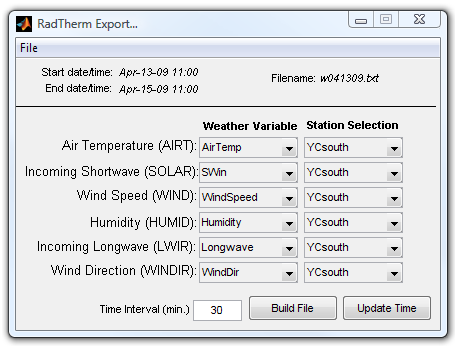
\includegraphics[width=0.48\linewidth]{\YCfiles figures/radexport_b.png}\label{fig:radexport_b}}\quad
	\subfloat[]{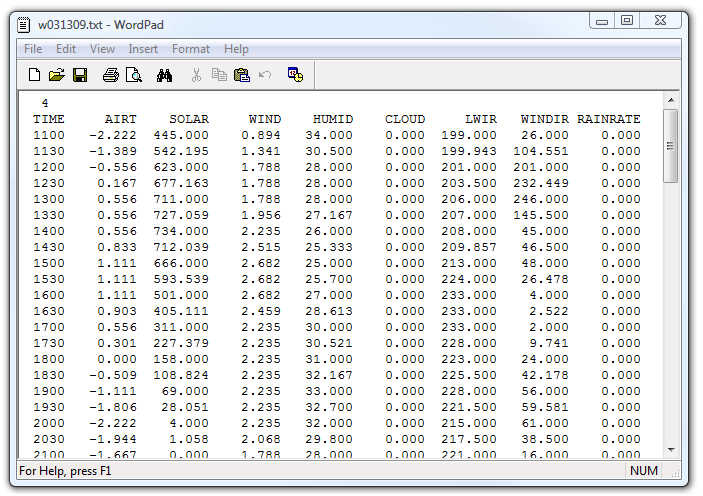
\includegraphics[width=0.48\linewidth]{\YCfiles figures/radexport_a.png}\label{fig:radexport_a}}
	\caption{(a) RadTherm/RT file exporter and (b) an example output file.}
	\label{fig:radexport}
\end{figure}

When using the exporter, begin by selecting the desired station from the right-column of pop-up menus.  When a station is selected the corresponding Weather Variable pop-up menu is changed to include weather variables with the necessary units.  The names that appear in both menus correspond to the tags assigned to the *.yc file for the stations, as discussed in Section \ref{sec:advanced}.  The start and end date/time values may be changed using the Program Control window and then by pressing the Update Time button.  Finally, the file is created by pressing Build File, a prompt will open for selecting the location to save the file.  The filename is dictated by the date.

The RadTherm/RT exporter also allows for the configuration of the pop-up menus to be saved.  This is available from the File menu on the exporter via the Save and Open Settings options.  These settings files utilize a *.rdt extension.
